\documentclass[11pt,a4paper]{article}

\usepackage[provide=*,french]{babel}
\usepackage[a4paper,margin=2.4cm,headheight=14pt]{geometry}
\usepackage{amsmath}
\usepackage{fontspec}
\usepackage{unicode-math}
\setmainfont{Latin Modern Roman}
\setsansfont{Latin Modern Sans}
\setmonofont{Latin Modern Mono}
\setmathfont{Latin Modern Math}
\usepackage{booktabs,tabularx,array}
\usepackage{graphicx}
\usepackage{caption}
\usepackage{xcolor}
\usepackage{fancyhdr}
\usepackage{enumitem}
\usepackage[hidelinks]{hyperref}

% Generated by report/make_numbers.py -- do not edit by hand.
\newcommand{\testgcnthree}{63,04}
\newcommand{\testsdgcnthree}{3,29}
\newcommand{\testmingcnthree}{59,25}
\newcommand{\testmaxgcnthree}{65,11}
\newcommand{\valgcnthree}{62,49}
\newcommand{\valsdgcnthree}{3,30}
\newcommand{\traingcnthree}{62,66}
\newcommand{\seedsgcnthree}{3}
\newcommand{\testcellgcnthree}{63,04\pmv{}3,29}
\newcommand{\valcellgcnthree}{62,49\pmv{}3,30}
\newcommand{\paramsgcnthree}{33\,994}
\newcommand{\bestepgcnthree}{20,0}
\newcommand{\secgcnthree}{9}
\newcommand{\mingcnthree}{3}
\newcommand{\testgcn}{72,39}
\newcommand{\testsdgcn}{6,68}
\newcommand{\testmingcn}{64,67}
\newcommand{\testmaxgcn}{76,35}
\newcommand{\valgcn}{72,53}
\newcommand{\valsdgcn}{6,44}
\newcommand{\traingcn}{72,21}
\newcommand{\seedsgcn}{3}
\newcommand{\testcellgcn}{72,39\pmv{}6,68}
\newcommand{\valcellgcn}{72,53\pmv{}6,44}
\newcommand{\paramsgcn}{34\,122}
\newcommand{\bestepgcn}{20,0}
\newcommand{\secgcn}{9}
\newcommand{\mingcn}{3}
\newcommand{\testsageraw}{75,76}
\newcommand{\testsdsageraw}{2,86}
\newcommand{\testminsageraw}{73,75}
\newcommand{\testmaxsageraw}{79,03}
\newcommand{\valsageraw}{75,21}
\newcommand{\valsdsageraw}{2,71}
\newcommand{\trainsageraw}{75,07}
\newcommand{\seedssageraw}{3}
\newcommand{\testcellsageraw}{75,76\pmv{}2,86}
\newcommand{\valcellsageraw}{75,21\pmv{}2,71}
\newcommand{\paramssageraw}{59\,018}
\newcommand{\bestepsageraw}{19,3}
\newcommand{\secsageraw}{7}
\newcommand{\minsageraw}{2}
\newcommand{\testsage}{92,29}
\newcommand{\testsdsage}{0,17}
\newcommand{\testminsage}{92,09}
\newcommand{\testmaxsage}{92,39}
\newcommand{\valsage}{91,77}
\newcommand{\valsdsage}{0,28}
\newcommand{\trainsage}{92,03}
\newcommand{\seedssage}{3}
\newcommand{\testcellsage}{92,29\pmv{}0,17}
\newcommand{\valcellsage}{91,77\pmv{}0,28}
\newcommand{\paramssage}{59\,018}
\newcommand{\bestepsage}{19,0}
\newcommand{\secsage}{8}
\newcommand{\minsage}{3}
\newcommand{\testlenet}{99,10}
\newcommand{\testsdlenet}{0,10}
\newcommand{\testminlenet}{98,99}
\newcommand{\testmaxlenet}{99,19}
\newcommand{\vallenet}{99,07}
\newcommand{\valsdlenet}{0,01}
\newcommand{\trainlenet}{99,95}
\newcommand{\seedslenet}{3}
\newcommand{\testcelllenet}{99,10\pmv{}0,10}
\newcommand{\valcelllenet}{99,07\pmv{}0,01}
\newcommand{\paramslenet}{61\,706}
\newcommand{\besteplenet}{17,7}
\newcommand{\seclenet}{3}
\newcommand{\minlenet}{1}
\newcommand{\testcnn}{99,31}
\newcommand{\testsdcnn}{0,08}
\newcommand{\testmincnn}{99,26}
\newcommand{\testmaxcnn}{99,41}
\newcommand{\valcnn}{99,16}
\newcommand{\valsdcnn}{0,02}
\newcommand{\traincnn}{99,88}
\newcommand{\seedscnn}{3}
\newcommand{\testcellcnn}{99,31\pmv{}0,08}
\newcommand{\valcellcnn}{99,16\pmv{}0,02}
\newcommand{\paramscnn}{421\,642}
\newcommand{\bestepcnn}{15,7}
\newcommand{\seccnn}{3}
\newcommand{\mincnn}{1}
\newcommand{\worstclassgcn}{5}
\newcommand{\worstrecallgcn}{40,99}
\newcommand{\bestclassgcn}{1}
\newcommand{\bestrecallgcn}{96,48}
\newcommand{\worstclasssage}{9}
\newcommand{\worstrecallsage}{87,41}
\newcommand{\bestclasssage}{1}
\newcommand{\bestrecallsage}{98,15}
\newcommand{\worstclasslenet}{8}
\newcommand{\worstrecalllenet}{98,60}
\newcommand{\bestclasslenet}{0}
\newcommand{\bestrecalllenet}{99,59}
\newcommand{\worstclasscnn}{9}
\newcommand{\worstrecallcnn}{98,38}
\newcommand{\bestclasscnn}{1}
\newcommand{\bestrecallcnn}{99,88}
\newcommand{\recalltable}{Modèle & 0 & 1 & 2 & 3 & 4 & 5 & 6 & 7 & 8 & 9 \\ \midrule
GCN & 84,1 & 96,5 & 63,9 & 70,9 & 75,0 & 41,0 & 82,4 & 80,5 & 59,3 & 64,1 \\
GraphSAGE & 97,2 & 98,1 & 91,0 & 91,0 & 91,1 & 88,9 & 96,3 & 90,6 & 90,4 & 87,4 \\
LeNet-5 & 99,6 & 99,4 & 99,5 & 99,3 & 99,1 & 98,8 & 98,7 & 99,4 & 98,6 & 98,6 \\
CNN & 99,7 & 99,9 & 99,6 & 99,5 & 99,4 & 99,2 & 99,1 & 99,0 & 99,2 & 98,4 \\}
\newcommand{\confpaira}{9~$\to$~4}
\newcommand{\confcounta}{57}
\newcommand{\confpairb}{4~$\to$~9}
\newcommand{\confcountb}{56}
\newcommand{\confpairc}{7~$\to$~9}
\newcommand{\confcountc}{44}
\newcommand{\nodesmean}{65,7}
\newcommand{\nodesmin}{52}
\newcommand{\nodesmax}{81}
\newcommand{\edgesmean}{189,2}
\newcommand{\degreemean}{5,75}
\newcommand{\fmeanmeanintensity}{0,093}
\newcommand{\fstdmeanintensity}{0,240}
\newcommand{\fmeanx}{0,460}
\newcommand{\fstdx}{0,297}
\newcommand{\fmeany}{0,465}
\newcommand{\fstdy}{0,290}
\newcommand{\fmeanarea}{0,015}
\newcommand{\fstdarea}{0,005}
\newcommand{\fmeanstdintensity}{0,048}
\newcommand{\fstdstdintensity}{0,091}


\setlist{itemsep=2pt,topsep=4pt}
\captionsetup{font=small,labelfont=bf}
\pagestyle{fancy}
\fancyhf{}
\fancyhead[L]{\small Image-to-Graph Conversion and Classification using GNNs}
\fancyhead[R]{\small A.~Belloir}
\fancyfoot[C]{\thepage}
\renewcommand{\headrulewidth}{0.4pt}
\newcommand{\pct}{\,\%}
\newcommand{\pmv}{\,\ensuremath{\pm}\,}

\begin{document}

% ------------------------------------------------------------------ couverture
\begin{titlepage}
\centering
{\large Université Galatasaray\\Faculté d'Ingénierie et de Technologie\\Département de Génie Informatique\par}
\vspace{1.6cm}
{\large INF494 -- Projet de fin d'études\par}
\vspace{1.2cm}
{\LARGE\bfseries Classification d'images par réseaux de neurones sur graphes de superpixels\par}
\vspace{0.6cm}
{\large Image-to-Graph Conversion and Classification using GNNs\par}
\vspace{0.2cm}
{\normalsize\itshape Graf Sinir Ağları Kullanarak Görüntüden Grafa Dönüşüm ve Sınıflandırma\par}
\vspace{2cm}
\begin{tabular}{ll}
Étudiant & Axel Belloir \\
Encadrante & Ayşegül Tüysüz Erman \\
Année universitaire & 2025--2026 \\
\end{tabular}
\vfill
{\large Rapport remis en juin 2026 -- version révisée, novembre 2026\par}
\vspace{0.4cm}
{\small Code : \url{https://github.com/akselDang/INF494_projet}\par}
\end{titlepage}

% ------------------------------------------------------------------ résumé
\section*{Résumé}
Ce projet classe des images en les représentant non plus comme une grille de pixels, mais comme un graphe :
chaque image est découpée en superpixels par l'algorithme SLIC, chaque superpixel devient un nœud décrit par
cinq caractéristiques (intensité, position, aire, texture), et deux superpixels voisins sont reliés par une arête.
Un réseau de neurones sur graphes (GCN ou GraphSAGE, PyTorch Geometric) classe ensuite le graphe.

Sur MNIST, chaque modèle est sélectionné sur un jeu de validation, avec le même budget (20 époques) pour
tous et trois graines par configuration. L'exactitude moyenne en test est de \textbf{\testsage\pct} pour
GraphSAGE, contre \testgcn\pct{} pour GCN. Sur les pixels, un CNN de type LeNet-5, qui a à peu près le même nombre de paramètres
que GraphSAGE, atteint \testlenet\pct, et un CNN sept fois plus grand \testcnn\pct. Les modèles sur graphes
apprennent aussi beaucoup plus lentement : à la fin du budget, GCN progresse encore nettement, et son résultat varie
fortement d'une graine à l'autre. Sans standardisation des caractéristiques des nœuds, GraphSAGE tombe à
\testsageraw\pct.

\noindent\textbf{Mots-clés :} réseaux de neurones sur graphes, superpixels, SLIC, GCN, GraphSAGE, MNIST, PyTorch Geometric.

\vspace{0.5cm}
\noindent\fcolorbox{gray!60}{gray!8}{\parbox{\dimexpr\linewidth-2\fboxsep-2\fboxrule}{\small
\textbf{À propos de cette version.} Ce document révise le rapport remis en juin 2026. En novembre 2026, le code a été
restructuré et les expériences MNIST ont été relancées avec un protocole plus rigoureux : la meilleure époque est
choisie sur un jeu de validation et non plus sur le jeu de test, et tous les modèles ont le même budget
d'entraînement. Chaque configuration est entraînée avec trois graines, sur un GPU de Google Colab. Les chiffres de ce rapport remplacent ceux de juin. Les sections de gestion de projet du rapport d'origine
(planning, coûts, analyse SWOT) ne sont pas reprises.}}

\newpage
\tableofcontents
\newpage

% ------------------------------------------------------------------ 1
\section{Introduction}

Les réseaux de neurones convolutifs (CNN) dominent la classification d'images depuis LeCun et
al.~\cite{lecun1998} et Krizhevsky et al.~\cite{krizhevsky2012}. Ils supposent que l'image est une grille régulière
de pixels. Les réseaux de neurones sur graphes (GNN) relâchent cette hypothèse : ils travaillent sur des nœuds reliés
par des arêtes quelconques. Ce projet étudie une représentation intermédiaire : l'image est résumée par quelques
dizaines de régions homogènes, les superpixels, reliées selon leur voisinage.

\paragraph{Objectifs.}
\begin{enumerate}
  \item Construire un pipeline reproductible qui transforme une image en graphe PyTorch Geometric.
  \item Comparer deux GNN, GCN et GraphSAGE, sur ces graphes.
  \item Mesurer l'effet des caractéristiques des nœuds : leur nombre (3 contre 5) et leur standardisation.
  \item Situer les GNN face à des CNN sur les pixels, à nombre de paramètres comparable (LeNet-5) et supérieur.
  \item Analyser les erreurs : exactitude par classe, matrices de confusion, exemples mal classés.
\end{enumerate}

Le jeu de données principal est MNIST~\cite{lecun1998} : 70\,000 images de chiffres manuscrits en niveaux de gris,
de taille $28\times28$. Le code prend aussi en charge CIFAR-10 (section~\ref{sec:conclusion}).

% ------------------------------------------------------------------ 2
\section{État de l'art}

\paragraph{Réseaux de neurones sur graphes.}
Les GNN ont été introduits par Gori et al.~\cite{gori2005}. Gilmer et al.~\cite{gilmer2017} ont unifié la plupart
des architectures dans le cadre du passage de messages : à chaque couche, chaque nœud agrège les représentations de
ses voisins puis met à jour la sienne.

\paragraph{GCN.} Kipf et Welling~\cite{kipf2017} définissent la couche
\begin{equation}
H^{(l+1)} = \sigma\bigl(\tilde D^{-1/2}\tilde A\,\tilde D^{-1/2} H^{(l)} W^{(l)}\bigr),
\label{eq:gcn}
\end{equation}
où $\tilde A = A + I$ est la matrice d'adjacence avec boucles et $\tilde D$ sa matrice des degrés.
Chaque nœud devient une moyenne pondérée de lui-même et de ses voisins, avec \emph{les mêmes poids} $W^{(l)}$ pour tous.

\paragraph{GraphSAGE.} Hamilton et al.~\cite{hamilton2017} séparent la représentation du nœud de celle de son voisinage :
\begin{equation}
h_v^{(l+1)} = \sigma\Bigl(W_1^{(l)} h_v^{(l)} + W_2^{(l)} \tfrac{1}{|\mathcal N(v)|}\textstyle\sum_{u\in\mathcal N(v)} h_u^{(l)}\Bigr),
\label{eq:sage}
\end{equation}
ce qui équivaut à appliquer une couche linéaire à la concaténation $[h_v \,\|\, \mathrm{moyenne}_{u}\,h_u]$.
Le nœud garde ainsi sa propre information au lieu de la diluer dans celle de ses voisins.

\paragraph{Attention.} Les Graph Attention Networks de Veličković et al.~\cite{velickovic2018} apprennent un poids
par voisin ; ils ne sont pas utilisés ici.

\paragraph{Superpixels.} SLIC~\cite{achanta2012} regroupe les pixels par un $k$-moyennes local dans l'espace
(couleur, position), avec la distance
\begin{equation}
D = \sqrt{d_c^2 + \Bigl(\frac{d_s}{S}\Bigr)^2 m^2},\qquad S = \sqrt{N/K},
\end{equation}
où $d_c$ et $d_s$ sont les distances de couleur et de position, $N$ le nombre de pixels, $K$ le nombre de superpixels
visé et $m$ la compacité : plus $m$ est petit, plus les superpixels suivent les contours.

\paragraph{GNN sur superpixels.} Monti et al.~\cite{monti2017} ont introduit la classification de MNIST représenté
par 75 superpixels, où leur modèle MoNet atteint 91,11\pct. Knyazev et al.~\cite{knyazev2019} utilisent ces graphes
pour étudier l'attention dans les GNN. Le banc d'essai de Dwivedi et al.~\cite{dwivedi2023} construit des graphes de
75 superpixels SLIC au plus, reliés aux 8 plus proches voisins, avec l'intensité et la position comme caractéristiques ;
à environ 100\,000 paramètres, GCN y atteint 90,71\pct{} et GraphSAGE 97,31\pct. Nos graphes sont construits
différemment (adjacence des régions, cinq caractéristiques, budget de paramètres plus faible) : ces chiffres donnent
un ordre de grandeur, pas une comparaison directe.

% ------------------------------------------------------------------ 3
\section{Méthode}

\subsection{De l'image au graphe}

\paragraph{Segmentation.} Chaque image est segmentée par SLIC (\texttt{scikit-image}) avec $K = 75$ superpixels visés
et une compacité $m = 0{,}1$, adaptée à des intensités dans $[0,1]$. Le nombre de superpixels obtenu varie d'une image
à l'autre : \nodesmean{} en moyenne sur l'ensemble d'entraînement, entre \nodesmin{} et \nodesmax.
SLIC est déterministe : la même image donne toujours la même segmentation.

\paragraph{Caractéristiques des nœuds.} Chaque superpixel devient un nœud décrit par cinq caractéristiques
(tableau~\ref{tab:features}).

\begin{table}[h]
\centering\small
\caption{Caractéristiques des nœuds sur MNIST, avec leur moyenne et leur écart-type bruts sur l'ensemble d'entraînement.}
\label{tab:features}
\begin{tabular}{lllcc}
\toprule
\# & Caractéristique & Définition & Moyenne & Écart-type \\
\midrule
1 & \texttt{mean\_intensity} & intensité moyenne du superpixel & \fmeanmeanintensity & \fstdmeanintensity \\
2 & \texttt{x} & abscisse du centre, divisée par la largeur & \fmeanx & \fstdx \\
3 & \texttt{y} & ordonnée du centre, divisée par la hauteur & \fmeany & \fstdy \\
4 & \texttt{area} & part de l'image couverte & \fmeanarea & \fstdarea \\
5 & \texttt{std\_intensity} & écart-type de l'intensité (texture) & \fmeanstdintensity & \fstdstdintensity \\
\bottomrule
\end{tabular}
\end{table}

\paragraph{Arêtes.} Deux superpixels sont reliés s'ils se touchent, en voisinage de 8 pixels. C'est le graphe
d'adjacence des régions de \texttt{scikit-image} (\texttt{rag\_mean\_color}, connectivité 2), calculé ici directement
avec \texttt{numpy}. Chaque arête est stockée dans les deux sens. Un graphe compte en moyenne \edgesmean{} arêtes,
soit un degré moyen de \degreemean.

\paragraph{Standardisation.} Les échelles brutes sont très différentes : l'écart-type de l'aire est de \fstdarea,
contre \fstdmeanintensity{} pour l'intensité. Chaque caractéristique est donc centrée et réduite avec la moyenne et
l'écart-type calculés sur les seuls graphes d'entraînement, puis la même transformation est appliquée aux graphes de
validation et de test. L'effet de ce choix est mesuré à la section~\ref{sec:ablations}.

La figure~\ref{fig:pipeline} montre les trois étapes sur une image d'entraînement.

\begin{figure}[h]
\centering
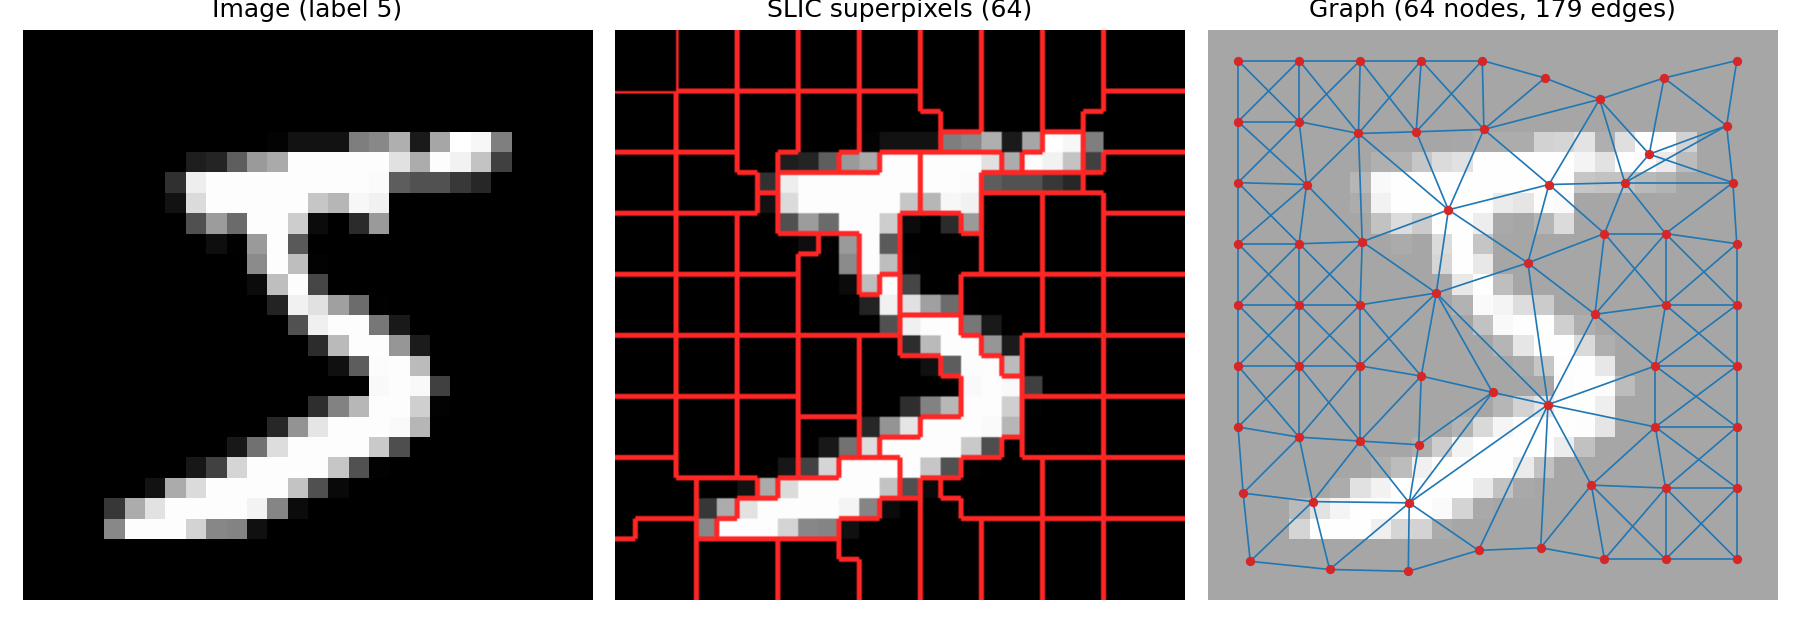
\includegraphics[width=\linewidth]{figures/mnist_pipeline_demo.png}
\caption{De l'image au graphe : image d'origine, superpixels SLIC, graphe (nœuds aux centres des superpixels).}
\label{fig:pipeline}
\end{figure}

\subsection{Modèles}

Les modèles sont implémentés avec PyTorch Geometric~\cite{fey2019}. Les deux GNN partagent la même structure : trois couches de convolution sur graphe (5 $\to$ 64 $\to$ 128 $\to$ 128),
chacune suivie d'une ReLU, une moyenne sur tous les nœuds du graphe
$h_G = \frac{1}{N}\sum_{v=1}^{N} h_v^{(3)}$, puis un perceptron $128 \to 64 \to 10$ avec un dropout de 0,5.
Seule la couche de convolution change : équation~\eqref{eq:gcn} pour GCN, \eqref{eq:sage} pour GraphSAGE.
Après trois couches, chaque nœud a intégré l'information des nœuds situés à au plus trois arêtes.

Deux CNN sur les pixels servent de référence :
\begin{itemize}
  \item \textbf{LeNet-5}~\cite{lecun1998} : deux convolutions $5\times5$ et trois couches denses, avec un nombre de paramètres proche de celui de GraphSAGE ;
  \item \textbf{CNN} : deux convolutions $3\times3$ (32 et 64 filtres) et une couche dense de 128 neurones, avec dropout.
\end{itemize}

\begin{table}[h]
\centering\small
\caption{Modèles comparés.}
\label{tab:models}
\begin{tabular}{llr}
\toprule
Modèle & Entrée & Paramètres \\
\midrule
GCN & graphe & \paramsgcn \\
GraphSAGE & graphe & \paramssage \\
LeNet-5 & pixels & \paramslenet \\
CNN & pixels & \paramscnn \\
\bottomrule
\end{tabular}
\end{table}

% ------------------------------------------------------------------ 4
\section{Protocole expérimental}
\label{sec:protocol}

\begin{itemize}
  \item \textbf{Découpage.} Les 60\,000 images d'entraînement de MNIST sont séparées une fois pour toutes en
  55\,000 images d'entraînement et 5\,000 de validation. Le découpage est le même pour tous les modèles et toutes les
  graines. Les 10\,000 images de test ne servent à aucun choix.
  \item \textbf{Sélection.} À chaque époque, on mesure l'exactitude sur la validation ; on garde les poids de la
  meilleure époque. Le test est évalué une seule fois, avec ces poids.
  \item \textbf{Entraînement.} Mêmes réglages pour tous les modèles : Adam, taux d'apprentissage $10^{-3}$, décroissance
  des poids $10^{-4}$, lots de 64, 20 époques, taux divisé par deux toutes les 8 époques, entropie croisée.
  \item \textbf{Graines.} Chaque entraînement utilise une graine fixée, qui détermine l'initialisation et l'ordre
  des lots. Chaque configuration est entraînée avec les graines 0, 1 et 2 ; les tableaux donnent la moyenne
  \pmv{} l'écart-type (corrigé, $n = 3$). Avec trois graines, cet écart-type reste une estimation grossière.
  \item \textbf{Métriques.} Exactitude (part des images bien classées) et, pour chaque chiffre, rappel (part des images
  de ce chiffre bien classées).
  \item \textbf{Matériel.} GPU NVIDIA T4 (Google Colab) ; PyTorch 2.14, PyTorch Geometric 2.8. Une époque dure
  environ \secsage~s pour GraphSAGE et \seclenet~s pour LeNet-5.
\end{itemize}

Le budget de 20 époques avait été fixé pour un calcul sur CPU et a été conservé. Il est identique pour tous les modèles, ce qui rend la
comparaison équitable, mais les courbes de validation (figure~\ref{fig:curves}) indiquent si certains modèles auraient
profité d'un entraînement plus long.

% ------------------------------------------------------------------ 5
\section{Implémentation}

Le code est organisé en modules indépendants (tableau~\ref{tab:repo}). Chaque entraînement écrit un fichier JSON
(configuration, historique par époque, meilleure époque, exactitudes de validation et de test, versions des
bibliothèques), les prédictions sur le test et les meilleurs poids ; les tableaux et figures de ce rapport sont
produits à partir de ces fichiers.

\begin{table}[h]
\centering\small
\caption{Organisation du code.}
\label{tab:repo}
\begin{tabularx}{\linewidth}{lX}
\toprule
Fichier & Rôle \\
\midrule
\texttt{src/graphs.py} & segmentation SLIC, caractéristiques, arêtes, construction et cache des graphes \\
\texttt{src/data.py} & chargement de MNIST et CIFAR-10, découpage entraînement / validation \\
\texttt{src/models.py} & GCN, GraphSAGE, LeNet-5, CNN \\
\texttt{src/train.py} & entraînement, sélection sur la validation, évaluation unique sur le test \\
\texttt{src/summarize.py} & tableau des résultats (moyenne \pmv{} écart-type sur les graines) \\
\texttt{src/visualize.py} & matrices de confusion, rappel par classe, courbes, exemples d'erreurs \\
\texttt{src/demo\_pipeline.py} & figure du pipeline et statistiques des graphes \\
\texttt{run\_all.sh}, \texttt{run\_all.ps1} & toutes les expériences de ce rapport \\
\bottomrule
\end{tabularx}
\end{table}

\paragraph{Construction des graphes.} Les 70\,000 graphes sont construits une seule fois puis mis en cache.
Le calcul des arêtes, vectorisé avec \texttt{numpy}, donne exactement le même graphe que \texttt{rag\_mean\_color}
(vérifié sur 200 images) ; la construction complète prend quelques minutes sur 2 cœurs, contre environ deux heures
dans la première version du projet.

\paragraph{Lots de graphes.} PyTorch Geometric regroupe les graphes d'un lot en un seul grand graphe sans
connexion entre eux ; un vecteur \texttt{batch} indique à quel graphe appartient chaque nœud, ce qui permet la
moyenne par graphe même quand les graphes n'ont pas le même nombre de nœuds.

% ------------------------------------------------------------------ 6
\section{Résultats}
\label{sec:results}

\subsection{Comparaison des modèles}

\begin{table}[h]
\centering\small
\caption{Exactitude sur MNIST (\%). Meilleure époque choisie sur la validation ; test évalué une fois par
entraînement. Moyenne \pmv{} écart-type sur trois graines.}
\label{tab:results}
\begin{tabular}{llrccc}
\toprule
Modèle & Entrée & Paramètres & Graines & Validation & Test \\
\midrule
GCN & graphe & \paramsgcn & \seedsgcn & \valcellgcn & \testcellgcn \\
GraphSAGE & graphe & \paramssage & \seedssage & \valcellsage & \textbf{\testcellsage} \\
\midrule
LeNet-5 & pixels & \paramslenet & \seedslenet & \valcelllenet & \testcelllenet \\
CNN & pixels & \paramscnn & \seedscnn & \valcellcnn & \testcellcnn \\
\bottomrule
\end{tabular}
\end{table}

Parmi les modèles sur graphes, GraphSAGE est nettement meilleur : \testsage\pct{} en test contre
\testgcn\pct{} pour GCN, dans exactement les mêmes conditions. GraphSAGE est aussi très stable (écart-type de
\testsdsage{} point), alors que GCN varie de \testmingcn\pct{} à \testmaxgcn\pct{} selon la graine. Les deux
CNN, qui travaillent sur les pixels, restent devant : \testlenet\pct{} pour LeNet-5 et \testcnn\pct{} pour le
CNN. L'écart de 0,2 point entre les deux CNN est de l'ordre de deux écarts-types : trois graines ne suffisent pas
à conclure. Les écarts entre familles de modèles, de 7 à 27 points, dépassent largement la variation entre graines.

Les modèles sur graphes ne surapprennent pas : leur exactitude d'entraînement, mesurée en mode évaluation, est
proche de celle du test (\trainsage\pct{} contre \testsage\pct{} pour GraphSAGE, \traingcn\pct{} contre
\testgcn\pct{} pour GCN). Ils sont limités par ce qu'ils parviennent à apprendre dans le budget, pas par la
généralisation. La figure~\ref{fig:curves} le confirme : LeNet-5 atteint environ 96\pct{} de validation dès la
première époque, alors que GraphSAGE n'atteint sa meilleure validation que vers l'époque 19 en moyenne et que GCN
gagne encore de 0,5 à 1,2 point par époque sur les cinq dernières, selon la graine. Ces chiffres comparent donc les modèles à budget
égal ; avec un entraînement plus long, les GNN, et surtout GCN, s'amélioreraient.

\begin{figure}[h]
\centering
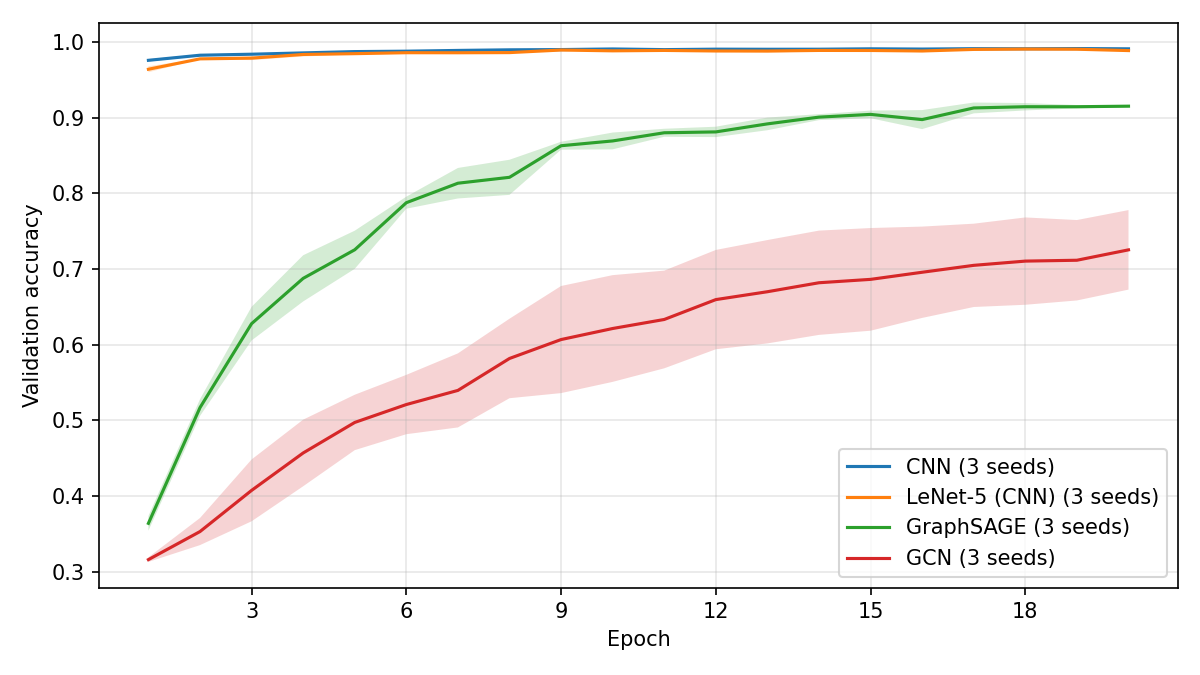
\includegraphics[width=0.82\linewidth]{figures/mnist_learning_curves.png}
\caption{Exactitude de validation par époque : moyenne sur trois graines, la bande indique l'écart-type.}
\label{fig:curves}
\end{figure}

\subsection{Ablations}
\label{sec:ablations}

\paragraph{Standardisation des caractéristiques.} La même configuration de GraphSAGE a été entraînée sans
standardisation (tableau~\ref{tab:ablation}). L'exactitude en test passe de \testsage\pct{} à
\testsageraw\pct, soit plus de 16 points de moins, et le résultat varie davantage d'une graine à l'autre.
L'apprentissage est surtout plus lent : après six époques, la validation est d'environ 46\pct{} sans
standardisation contre 79\pct{} avec, et elle progresse encore en fin de budget. C'est cohérent avec les échelles
du tableau~\ref{tab:features} : l'aire varie environ cinquante fois moins que l'intensité, si bien que, sans
standardisation, elle n'influence presque pas la première couche.

\paragraph{Nombre de caractéristiques.} GCN a été entraîné avec les trois premières caractéristiques seulement
(intensité moyenne et position), sans l'aire ni l'écart-type de l'intensité. Il obtient \testgcnthree\pct{} en
test contre \testgcn\pct{} avec les cinq, soit environ 9 points de moins en moyenne. Les écarts-types sont
cependant élevés (\testsdgcnthree{} et \testsdgcn{} points) et les plages se recouvrent : de
\testmingcnthree\pct{} à \testmaxgcnthree\pct{} avec trois caractéristiques, de \testmingcn\pct{} à
\testmaxgcn\pct{} avec cinq. Avec trois graines et un GCN qui n'a pas convergé, c'est une tendance, pas une
conclusion ferme.

\begin{table}[h]
\centering\small
\caption{Ablations sur MNIST : exactitude (\%), moyenne \pmv{} écart-type sur trois graines.}
\label{tab:ablation}
\begin{tabular}{llcc}
\toprule
Modèle & Caractéristiques & Validation & Test \\
\midrule
GraphSAGE & 5, standardisées & \valcellsage & \testcellsage \\
GraphSAGE & 5, non standardisées & \valcellsageraw & \testcellsageraw \\
\midrule
GCN & 5, standardisées & \valcellgcn & \testcellgcn \\
GCN & 3, standardisées & \valcellgcnthree & \testcellgcnthree \\
\bottomrule
\end{tabular}
\end{table}

\subsection{Analyse par classe}

\begin{table}[h]
\centering\small
\caption{Rappel par chiffre sur le test (\%, moyenne sur trois graines).}
\label{tab:recall}
\setlength{\tabcolsep}{4.5pt}
\begin{tabular}{lcccccccccc}
\toprule
\recalltable
\bottomrule
\end{tabular}
\end{table}

Les deux CNN dépassent 98\pct{} de rappel sur tous les chiffres (tableau~\ref{tab:recall}). GraphSAGE
va de \worstrecallsage\pct{} pour le \worstclasssage{} à \bestrecallsage\pct{} pour le \bestclasssage. Ses
confusions les plus fréquentes sont \confpaira{} (\confcounta{} images en moyenne par graine), \confpairb{} (\confcountb) et
\confpairc{} (\confcountc) : des chiffres dont les traits principaux se ressemblent, et que le résumé en
superpixels rapproche encore. GCN a beaucoup plus de mal, en particulier sur le 5 et le 8. La
figure~\ref{fig:confusion} compare les matrices de confusion de LeNet-5 et de GraphSAGE, deux modèles de taille
comparable, et la figure~\ref{fig:errors} montre des images mal classées par GraphSAGE avec leurs superpixels.

\begin{figure}[h]
\centering
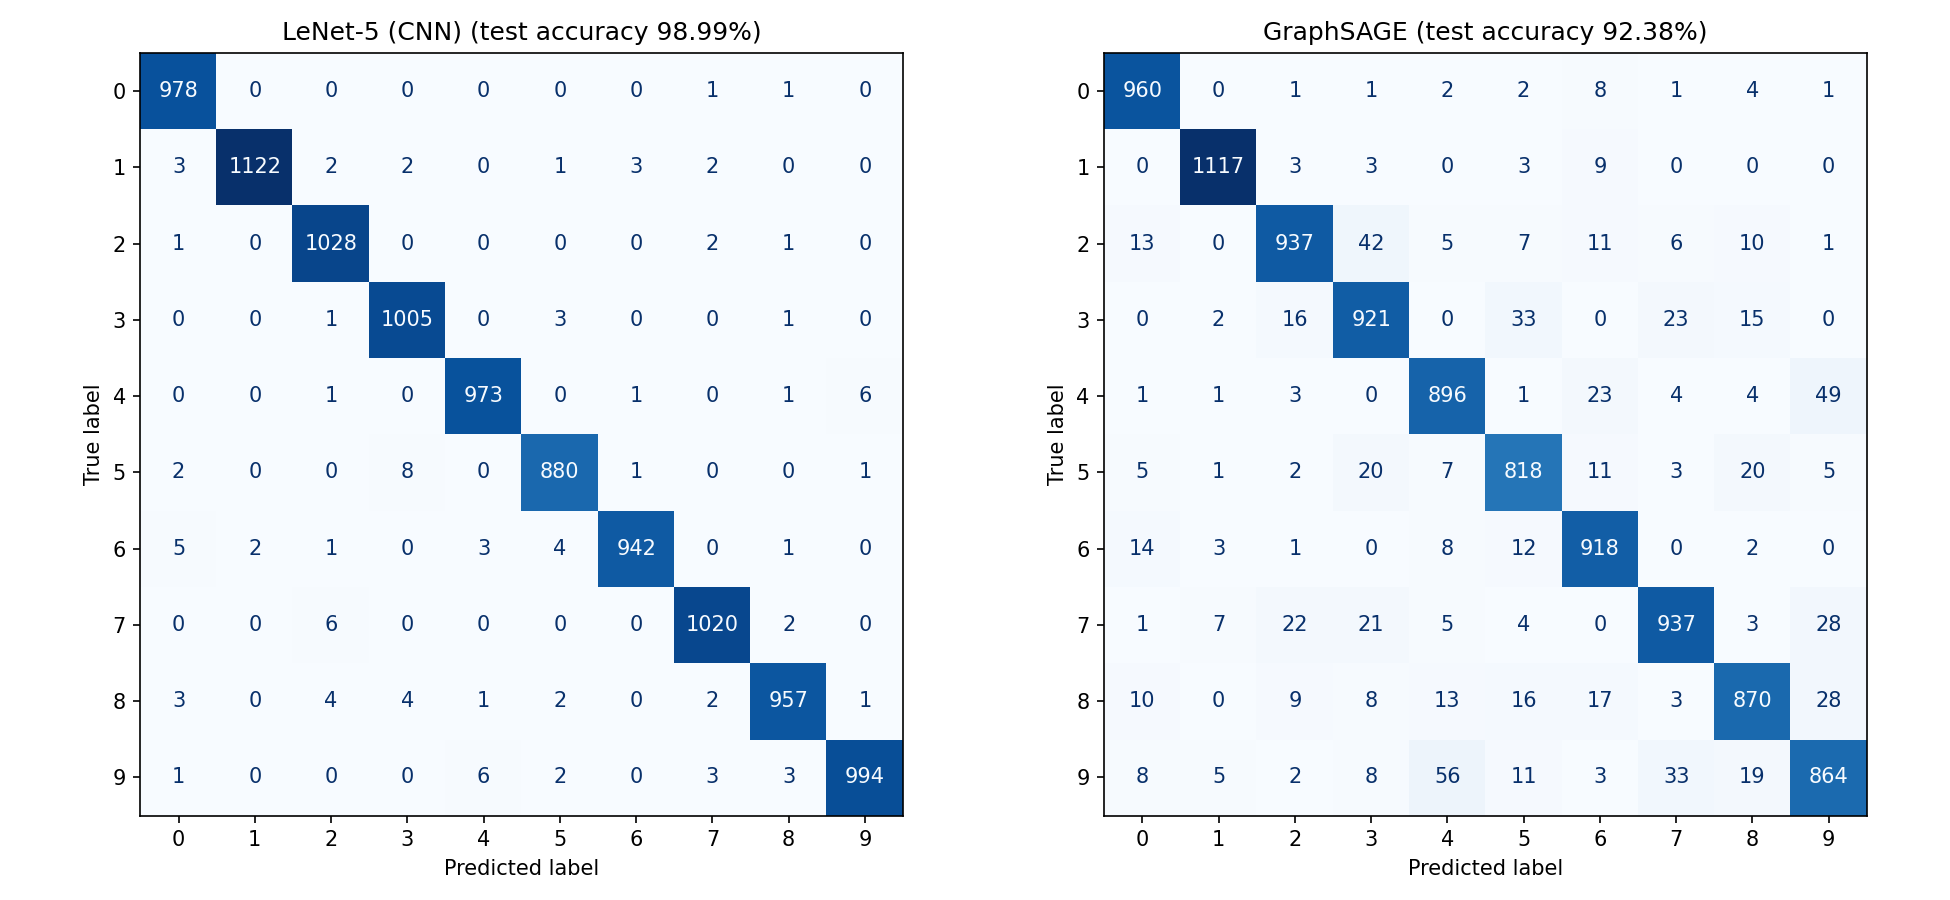
\includegraphics[width=\linewidth]{figures/mnist_confusion.png}
\caption{Matrices de confusion sur le test : LeNet-5 (gauche) et GraphSAGE (droite), graine 0.}
\label{fig:confusion}
\end{figure}

\begin{figure}[h]
\centering
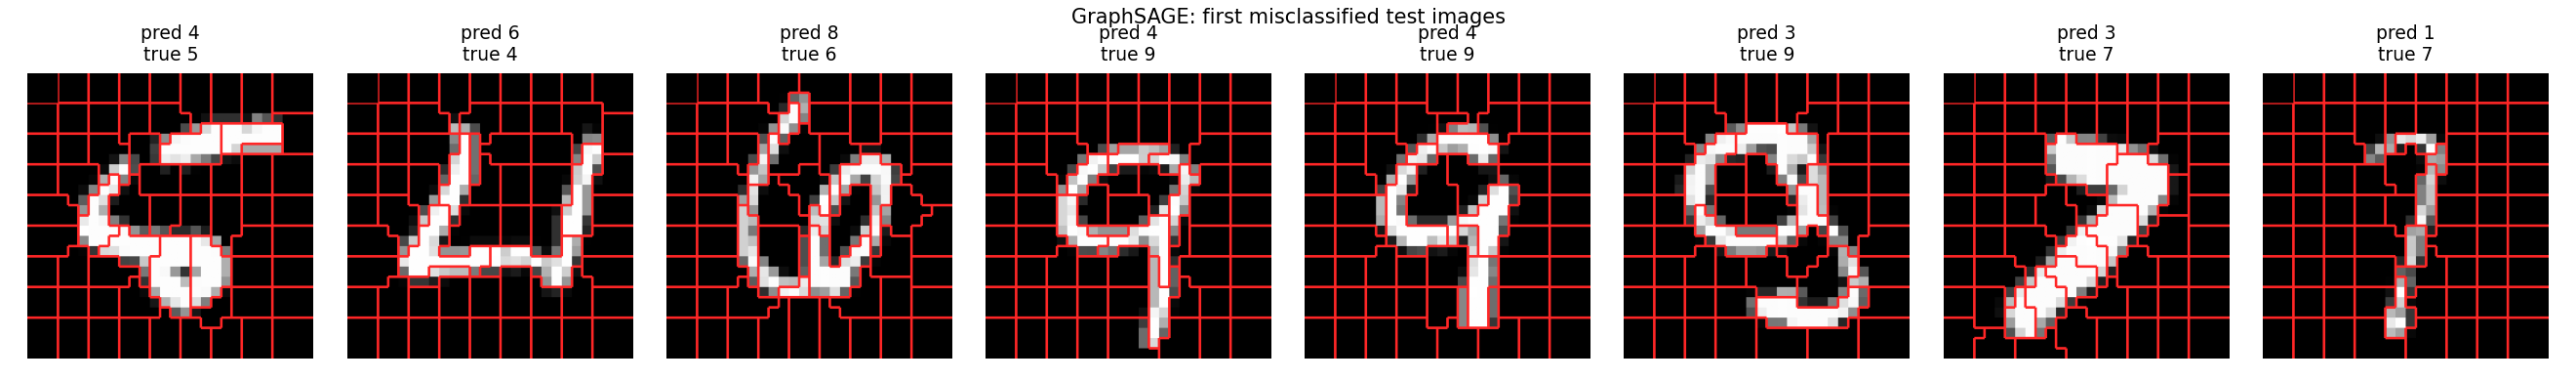
\includegraphics[width=\linewidth]{figures/mnist_errors_sage.png}
\caption{Premières images de test mal classées par GraphSAGE (graine 0), avec leurs superpixels.}
\label{fig:errors}
\end{figure}

% ------------------------------------------------------------------ 7
\section{Discussion}

\paragraph{Pourquoi GraphSAGE fait mieux que GCN.} Dans une couche GCN (équation~\eqref{eq:gcn}), un nœud
est remplacé par une moyenne de lui-même et de ses voisins, avec les mêmes poids pour tous. Avec environ six
voisins par nœud, sa propre information (position, intensité) ne pèse que pour une part sur sept environ, et elle
se dilue encore au fil des trois couches. GraphSAGE (équation~\eqref{eq:sage}) garde des poids séparés pour le
nœud et pour ses voisins : il peut distinguer « ce superpixel est clair » de « ses voisins sont clairs ». Le même
écart apparaît chez Dwivedi et al.~\cite{dwivedi2023} (90,71\pct{} pour GCN contre 97,31\pct{} pour
GraphSAGE) ; ici, GCN apprend en plus beaucoup plus lentement, et de façon instable d'une graine à l'autre.

\paragraph{Pourquoi les CNN restent devant.} La comparaison avec LeNet-5 montre que l'écart ne vient pas du
nombre de paramètres : à taille comparable, le CNN sur pixels gagne 7 points. Trois raisons y contribuent.
D'abord, la représentation : un graphe d'environ 66 superpixels décrits par cinq nombres résume l'image, et le
tracé fin du chiffre est remplacé par des moyennes par région. Ensuite, la moyenne finale sur tous les nœuds
donne le même poids au fond et au tracé, alors que la plupart des superpixels sont du fond (l'intensité moyenne
d'un nœud n'est que de \fmeanmeanintensity) ; la position des régions n'est plus connue qu'à travers les
coordonnées incluses dans les caractéristiques. Enfin, les GNN apprennent plus lentement et sont pénalisés par
un budget de 20 époques.

\paragraph{Comparaison avec la version de juin.} En juin, GraphSAGE atteignait 94,07\pct{} et GCN 77,54\pct.
Ces chiffres étaient optimistes, puisque la meilleure époque était choisie sur le test, et ils correspondaient à
des budgets d'entraînement plus longs et différents d'un modèle à l'autre. Ils ne sont pas comparables à ceux de
ce rapport.

\paragraph{Comparaison avec la littérature.} Dwivedi et al.~\cite{dwivedi2023} obtiennent 97,31\pct{} avec
GraphSAGE sur MNIST en superpixels, contre \testsage\pct{} ici. Leurs graphes relient chaque superpixel à ses
8 plus proches voisins, leurs modèles ont environ 100\,000 paramètres et 4 couches, et ils sont entraînés
beaucoup plus longtemps. L'écart est donc attendu et ne permet pas de juger notre construction des graphes
en elle-même.

\paragraph{Limites.} Trois graines seulement, ce qui donne des écarts-types peu précis, surtout pour GCN ;
20 époques, insuffisantes pour que GCN converge ; un seul jeu de données, CIFAR-10 n'ayant pas été relancé.

% ------------------------------------------------------------------ 9
\section{Conclusion et perspectives}
\label{sec:conclusion}

Ce projet construit un pipeline complet qui transforme une image en graphe de superpixels et le classe
avec un GNN, et il compare ce pipeline à des CNN avec un protocole d'évaluation propre : sélection sur un jeu de
validation, test évalué une seule fois, même budget pour tous les modèles. Sur MNIST, en moyenne sur trois
graines, GraphSAGE atteint
\testsage\pct{} et dépasse nettement GCN (\testgcn\pct), ce qui montre l'intérêt de garder l'information propre
de chaque nœud. Les CNN restent meilleurs, y compris à nombre de paramètres égal (\testlenet\pct{} pour LeNet-5) :
résumer l'image en superpixels fait perdre de l'information, et les GNN apprennent plus lentement.

Perspectives :
\begin{itemize}
  \item prolonger les entraînements jusqu'à la convergence de GCN et augmenter le nombre de graines ;
  \item enrichir les graphes : caractéristiques d'arêtes (distance, différence d'intensité), graphes des $k$ plus
  proches voisins comme Dwivedi et al. ;
  \item changer l'agrégation : attention (GAT), GIN, ou un pooling par attention plutôt que la moyenne, pour moins
  diluer le tracé dans le fond ;
  \item relancer CIFAR-10 avec ce protocole.
\end{itemize}

\begin{thebibliography}{99}\small
\bibitem{lecun1998} Y.~LeCun, L.~Bottou, Y.~Bengio, P.~Haffner. Gradient-based learning applied to document recognition. \emph{Proceedings of the IEEE}, 86(11):2278--2324, 1998.
\bibitem{krizhevsky2012} A.~Krizhevsky, I.~Sutskever, G.~E.~Hinton. ImageNet classification with deep convolutional neural networks. \emph{NeurIPS}, 2012.
\bibitem{gori2005} M.~Gori, G.~Monfardini, F.~Scarselli. A new model for learning in graph domains. \emph{IJCNN}, 2005.
\bibitem{gilmer2017} J.~Gilmer, S.~S.~Schoenholz, P.~F.~Riley, O.~Vinyals, G.~E.~Dahl. Neural message passing for quantum chemistry. \emph{ICML}, 2017.
\bibitem{kipf2017} T.~N.~Kipf, M.~Welling. Semi-supervised classification with graph convolutional networks. \emph{ICLR}, 2017.
\bibitem{hamilton2017} W.~L.~Hamilton, R.~Ying, J.~Leskovec. Inductive representation learning on large graphs. \emph{NeurIPS}, 2017.
\bibitem{velickovic2018} P.~Veličković, G.~Cucurull, A.~Casanova, A.~Romero, P.~Liò, Y.~Bengio. Graph attention networks. \emph{ICLR}, 2018.
\bibitem{achanta2012} R.~Achanta, A.~Shaji, K.~Smith, A.~Lucchi, P.~Fua, S.~Süsstrunk. SLIC superpixels compared to state-of-the-art superpixel methods. \emph{IEEE TPAMI}, 34(11):2274--2282, 2012.
\bibitem{monti2017} F.~Monti, D.~Boscaini, J.~Masci, E.~Rodolà, J.~Svoboda, M.~M.~Bronstein. Geometric deep learning on graphs and manifolds using mixture model CNNs. \emph{CVPR}, 2017.
\bibitem{knyazev2019} B.~Knyazev, G.~W.~Taylor, M.~R.~Amer. Understanding attention and generalization in graph neural networks. \emph{NeurIPS}, 2019.
\bibitem{dwivedi2023} V.~P.~Dwivedi, C.~K.~Joshi, A.~T.~Luu, T.~Laurent, Y.~Bengio, X.~Bresson. Benchmarking graph neural networks. \emph{JMLR}, 24(43):1--48, 2023.
\bibitem{fey2019} M.~Fey, J.~E.~Lenssen. Fast graph representation learning with PyTorch Geometric. \emph{ICLR Workshop on Representation Learning on Graphs and Manifolds}, 2019.
\end{thebibliography}

\end{document}
